
\documentclass[12pt,halfline,a4paper,]{ouparticle}

% Packages I think are necessary for basic Rmarkdown functionality
\usepackage{hyperref}
\usepackage{graphicx}
\usepackage{listings}
\usepackage{xcolor}
\usepackage{fancyvrb}
\usepackage{framed}

% Link coloring
\hypersetup{breaklinks=true,
            bookmarks=true,
            pdfauthor={},
            pdftitle={STA304XS - Assignment 3: Generalised Linear models}
            }


%% To allow better options for figure placement
%\usepackage{float}

% Packages that are supposedly required by OUP sty file
\usepackage{amssymb, amsmath, geometry, amsfonts, verbatim, endnotes, setspace}

% use upquote if available, for straight quotes in verbatim environments
\IfFileExists{upquote.sty}{\usepackage{upquote}}{}

% Macros for dealing with affiliations, footnotes, etc.
\makeatletter
\def\Newlabel#1#2#3{\expandafter\gdef\csname #1@#2\endcsname{#3}}

\def\Ref#1#2{\@ifundefined{#1@#2}{???}{\csname #1@#2\endcsname}}

\newcommand*\samethanks[1][\value{footnote}]{\footnotemark[#1]}

\newcommand*\ifcounter[1]{%
  \ifcsname c@#1\endcsname
    \expandafter\@firstoftwo
  \else
    \expandafter\@secondoftwo
  \fi
}

\newcommand*\thanksbycode[1]{%
  \ifcounter{FNCT@#1}
    {\samethanks[\value{FNCT@#1}]}
    {\thanks{\Ref{FN}{#1}}\newcounter{FNCT@#1}\setcounter{FNCT@#1}{\value{footnote}}}
}

% Create labels for Addresses if the are given in Elsevier format

% Create labels for Footnotes if the are given in Elsevier format

% Part for setting citation format package: natbib

% Part for setting citation format package: biblatex

% Pandoc syntax highlighting
\usepackage{color}
\usepackage{fancyvrb}
\newcommand{\VerbBar}{|}
\newcommand{\VERB}{\Verb[commandchars=\\\{\}]}
\DefineVerbatimEnvironment{Highlighting}{Verbatim}{commandchars=\\\{\}}
% Add ',fontsize=\small' for more characters per line
\usepackage{framed}
\definecolor{shadecolor}{RGB}{248,248,248}
\newenvironment{Shaded}{\begin{snugshade}}{\end{snugshade}}
\newcommand{\AlertTok}[1]{\textcolor[rgb]{0.94,0.16,0.16}{#1}}
\newcommand{\AnnotationTok}[1]{\textcolor[rgb]{0.56,0.35,0.01}{\textbf{\textit{#1}}}}
\newcommand{\AttributeTok}[1]{\textcolor[rgb]{0.13,0.29,0.53}{#1}}
\newcommand{\BaseNTok}[1]{\textcolor[rgb]{0.00,0.00,0.81}{#1}}
\newcommand{\BuiltInTok}[1]{#1}
\newcommand{\CharTok}[1]{\textcolor[rgb]{0.31,0.60,0.02}{#1}}
\newcommand{\CommentTok}[1]{\textcolor[rgb]{0.56,0.35,0.01}{\textit{#1}}}
\newcommand{\CommentVarTok}[1]{\textcolor[rgb]{0.56,0.35,0.01}{\textbf{\textit{#1}}}}
\newcommand{\ConstantTok}[1]{\textcolor[rgb]{0.56,0.35,0.01}{#1}}
\newcommand{\ControlFlowTok}[1]{\textcolor[rgb]{0.13,0.29,0.53}{\textbf{#1}}}
\newcommand{\DataTypeTok}[1]{\textcolor[rgb]{0.13,0.29,0.53}{#1}}
\newcommand{\DecValTok}[1]{\textcolor[rgb]{0.00,0.00,0.81}{#1}}
\newcommand{\DocumentationTok}[1]{\textcolor[rgb]{0.56,0.35,0.01}{\textbf{\textit{#1}}}}
\newcommand{\ErrorTok}[1]{\textcolor[rgb]{0.64,0.00,0.00}{\textbf{#1}}}
\newcommand{\ExtensionTok}[1]{#1}
\newcommand{\FloatTok}[1]{\textcolor[rgb]{0.00,0.00,0.81}{#1}}
\newcommand{\FunctionTok}[1]{\textcolor[rgb]{0.13,0.29,0.53}{\textbf{#1}}}
\newcommand{\ImportTok}[1]{#1}
\newcommand{\InformationTok}[1]{\textcolor[rgb]{0.56,0.35,0.01}{\textbf{\textit{#1}}}}
\newcommand{\KeywordTok}[1]{\textcolor[rgb]{0.13,0.29,0.53}{\textbf{#1}}}
\newcommand{\NormalTok}[1]{#1}
\newcommand{\OperatorTok}[1]{\textcolor[rgb]{0.81,0.36,0.00}{\textbf{#1}}}
\newcommand{\OtherTok}[1]{\textcolor[rgb]{0.56,0.35,0.01}{#1}}
\newcommand{\PreprocessorTok}[1]{\textcolor[rgb]{0.56,0.35,0.01}{\textit{#1}}}
\newcommand{\RegionMarkerTok}[1]{#1}
\newcommand{\SpecialCharTok}[1]{\textcolor[rgb]{0.81,0.36,0.00}{\textbf{#1}}}
\newcommand{\SpecialStringTok}[1]{\textcolor[rgb]{0.31,0.60,0.02}{#1}}
\newcommand{\StringTok}[1]{\textcolor[rgb]{0.31,0.60,0.02}{#1}}
\newcommand{\VariableTok}[1]{\textcolor[rgb]{0.00,0.00,0.00}{#1}}
\newcommand{\VerbatimStringTok}[1]{\textcolor[rgb]{0.31,0.60,0.02}{#1}}
\newcommand{\WarningTok}[1]{\textcolor[rgb]{0.56,0.35,0.01}{\textbf{\textit{#1}}}}

% tightlist command for lists without linebreak
\providecommand{\tightlist}{%
  \setlength{\itemsep}{0pt}\setlength{\parskip}{0pt}}



\usepackage{pdfpages}
\usepackage{booktabs}
\usepackage{longtable}
\usepackage{array}
\usepackage{multirow}
\usepackage{wrapfig}
\usepackage{float}
\usepackage{colortbl}
\usepackage{pdflscape}
\usepackage{tabu}
\usepackage{threeparttable}
\usepackage{threeparttablex}
\usepackage[normalem]{ulem}
\usepackage{makecell}
\usepackage{xcolor}

\begin{document}

\title{STA304XS - Assignment 3: Generalised Linear models}

\author{%
%
% Code for old style authors field
%
% Add \and if both authors and author
%
%
% Code for new (elsevier) style author field
\name{Jing Yeh}
%
\email{\href{mailto:yhxjin001@myuct.ac.za}{yhxjin001@myuct.ac.za}}%
%
%
%
\and
\name{Saurav Sathnarayan}
%
\email{\href{mailto:sthsau001@myuct.ac.za}{sthsau001@myuct.ac.za}}%
%
%
%
%
}

\abstract{This report explores the relationship between Ridge Logistic
Regression and Bayesian Maximum A Posteriori (MAP) estimation with
Gaussian priors. The theoretical connection between the ridge penalty
and the prior precision is derived, showing how regularisation arises
naturally from Bayesian assumptions. A modified Iteratively Weighted
Least Squares (IWLS) algorithm for ridge-penalised logistic regression
is derived step-by-step and implemented in R. The performance of the
custom Ridge-IWLS implementation is compared to standard software (e.g.,
glmnet), evaluating coefficient shrinkage, predictive accuracy, and
computational stability. The analysis highlights the role of
regularisation in improving generalisation and mitigating overfitting in
binary classification problems.}

\date{2025-10-23}

\keywords{Ridge Logistic Regression, Bayesian MAP Estimation, IWLS
Algorithm, Regularisation, Penalised Likelihood, Coefficient Shrinkage,
Logistic Regression, Generalisation.}

\maketitle




\includepdf[pages=1]{Department of Statistical Sciences - Plagiarism Declaration.pdf}
\newpage
\tableofcontents
\newpage

\section{Question 1 - Bayesian
Interpretation}\label{question-1---bayesian-interpretation}

\subsection{(a)}\label{a}

We start with the logistic regression model:

\[\Pr(Y_i = 1 \mid x_i) = \text{logit}^{-1}(x_i^\top \beta) = \dfrac{1}{1 + \exp(-x_i^\top \beta)}.\]

The log-likelihood for all \(n\) observations is

\[l(\beta) = \sum_{i=1}^n \left[ y_i x_i^\top \beta - \log(1 + e^{x_i^\top \beta}) \right].\]

Assume independent Normal priors for the coefficients:

\[\beta_j \sim N(0, \tau^2), \quad j = 1, \ldots, p.\]

Hence, the prior density is

\[\pi(\beta) = \prod_{j=1}^p \dfrac{1}{\sqrt{2\pi\tau^2}}
\exp\!\left(-\dfrac{\beta_j^2}{2\tau^2}\right)\]

Taking logs, we obtain the log-prior:

\[\log \pi(\beta) = -\dfrac{p}{2}\log(2\pi\tau^2)
-\dfrac{1}{2\tau^2}\sum_{j=1}^p \beta_j^2\]

Now, by Bayes' theorem,

\[\pi(\beta \mid y) = \dfrac{\pi(y \mid \beta)\, \pi(\beta)}{\pi(y)}\]

Taking logs of both sides gives

\[\log \pi(\beta \mid y) = \log \pi(y \mid \beta) + \log \pi(\beta) - \log \pi(y)\]

The term \(\log \pi(y)\) is a normalising constant that does not depend
on \(\beta\), so when maximising over \(\beta\), it can be ignored.
Therefore,

\[\log \pi(\beta \mid y) \propto \log \pi(y \mid \beta) + \log \pi(\beta)\]

Substituting the expressions for \(\log p(y \mid \beta)\) and
\(\log p(\beta)\), we have

\[\log p(\beta \mid y) \propto l(\beta) - \dfrac{1}{2\tau^2}\sum_{j=1}^p \beta_j^2\]

This is the expression for the log-posterior up to a constant. \newpage
To obtain the maximum a posteriori (MAP) estimate, we maximise
\(\log p(\beta \mid y)\) with respect to \(\beta\). Equivalently, we
minimise the negative log-posterior:

\[\widehat{\beta}_{MAP} = \arg\min_\beta
\left[ -l(\beta) + \dfrac{1}{2\tau^2}\sum_{j=1}^p \beta_j^2 \right]\]

If we define \(\lambda = \dfrac{1}{2\tau^2}\), then the optimisation
problem becomes

\[\boxed{
\widehat{\beta}_{MAP}
= \arg\min_\beta \left[ -l(\beta) + \lambda \|\beta\|_2^2 \right]
}\]

This shows that the MAP estimator under a Normal prior is equivalent to
the ridge-regularised logistic regression estimator, where the penalty
parameter \(\lambda\) corresponds to the precision of the prior.

\subsection{(b)}\label{b}

\textbf{Role of \(\lambda\) and \(\tau\):} \(\lambda\) controls the
amount of shrinkage or regularisation applied to the coefficients.A
\textbf{large \(\lambda\)} (small \(\tau^2\)) implies a strong prior
belief that coefficients should be close to zero, resulting in
\textbf{greater shrinkage}. A \textbf{small \(\lambda\)} (large
\(\tau^2\)) implies a weak prior, approaching the unpenalised
\textbf{maximum likelihood estimate (MLE)}.

\textbf{Effect of this regularisation:} It helps prevent
\textbf{overfitting} by penalising large coefficient values.

\textbf{Bayesian vs.~MLE perspective:} The MLE only uses the data and
can overfit when the sample size is small. The Bayesian (MAP) approach
incorporates \textbf{prior information} through \(\tau^2\), providing a
\textbf{probabilistic justification} for regularisation. Hence, the
Bayesian view explains \textbf{why} regularisation arises naturally as a
consequence of imposing a Gaussian prior.

\section{Question 2 - Deriving Ridge -
IWLS}\label{question-2---deriving-ridge---iwls}

\subsection{(a)}\label{a-1}

In IWLS, the weight for observation \(i\) is given by \[
w_i^{(t)} = \frac{1}{\operatorname{Var}(Y_i)} \left(\frac{\partial \mu_i}{\partial \eta_i}\right)^2.
\]

For logistic regression, \(\operatorname{Var}(Y_i) = p_i (1 - p_i)\) and
\(\frac{\partial \mu_i}{\partial \eta_i} = p_i (1 - p_i)\), so

\[
w_i^{(t)} = \frac{\left(p_i^{(t)} (1 - p_i^{(t)})\right)^2}{p_i^{(t)} (1 - p_i^{(t)})} 
= p_i^{(t)} (1 - p_i^{(t)}).
\]

These are exactly the diagonal entries of the weight matrix:

\[
W^{(t)} = \operatorname{diag}\Big(p_1^{(t)} (1 - p_1^{(t)}), \dots, p_n^{(t)} (1 - p_n^{(t)})\Big).
\]

and \(p^{(t)} = (p_1^{(t)}, \dots, p_n^{(t)})^\top\) are the predicted
probabilities at \(\beta^{(t)}\).

and for \(z^{(t)}\)

\[z_i^{(t)} = \eta_i^{(t)} + \frac{y_i - \mu_i^{(t)}}{\frac{\partial \mu_i}{\partial \eta_i}}\]

where \[
\eta_i^{(t)} = x_i^\top \beta^{(t)}, \quad \mu_i^{(t)} = \sigma(\eta_i^{(t)}) = p_i^{(t)}, \quad \frac{\partial \mu_i}{\partial \eta_i} = p_i^{(t)} (1 - p_i^{(t)}).
\]

Substituting the derivative for logistic regression gives

\[
z_i^{(t)} = x_i^\top \beta^{(t)} + \frac{y_i - p_i^{(t)}}{p_i^{(t)} (1 - p_i^{(t)})}.
\]

In matrix form, for all \(n\) observations:

\[
z^{(t)} = X \beta^{(t)} + (W^{(t)})^{-1} (y - p^{(t)}),
\]

From our IWLS formula, we have:

\[ (\textbf{X}^T \textbf{W}^{(t)} \textbf{X})^{-1} \beta^{(t+1)} = \textbf{X}^T \textbf{W}^{(t)} z^{(t)} \]
Thus,

\[\boxed{\beta^{(t+1)} = (\textbf{X}^T \textbf{W}^{(t)} \textbf{X})^{-1}\textbf{X}^T \textbf{W}^{(t)} z^{(t)}}   \]
\#\# (b)

We are asked to derive the modified IWLS update formula for the
Ridge-penalised objective function.

\begin{enumerate}
\def\labelenumi{\arabic{enumi}.}
\tightlist
\item
  Objective Function
\end{enumerate}

We start from the objective function to be minimised: \[
F(\boldsymbol{\beta}) = -\ell(\boldsymbol{\beta}) + \lambda \|\boldsymbol{\beta}\|_2^2 = -\ell(\boldsymbol{\beta}) + \lambda \boldsymbol{\beta}^\top \boldsymbol{\beta}
\] The Newton-Raphson update rule for minimising
\(F(\boldsymbol{\beta})\) is: \[
\boldsymbol{\beta}^{(t+1)} = \boldsymbol{\beta}^{(t)} - [H_F(\boldsymbol{\beta}^{(t)})]^{-1} U_F(\boldsymbol{\beta}^{(t)})
\] We need the gradient \(U_F\) and the Hessian \(H_F\) of our new
objective function \(F\).

\begin{enumerate}
\def\labelenumi{\arabic{enumi}.}
\setcounter{enumi}{2}
\tightlist
\item
  Gradient (\(U_F\)) and Hessian (\(H_F\))
\end{enumerate}

From part a, we know:

\begin{itemize}
  \item Standard Score Vector: $U_{\ell} = \frac{\partial \ell}{\partial \boldsymbol{\beta}} = \mathbf{X}^\top (\mathbf{y} - \mathbf{p})$

  \item Standard Hessian: $H_{\ell} = \frac{\partial^2 \ell}{\partial \boldsymbol{\beta} \partial \boldsymbol{\beta}^\top} = -\mathbf{X}^\top \mathbf{W} \mathbf{X}$

\end{itemize}

Now, we find the derivatives for our penalised objective \(F\):

Gradient (\(U_F\)):

\[U_F = \frac{\partial F}{\partial \boldsymbol{\beta}} = \frac{\partial}{\partial \boldsymbol{\beta}}(-\ell(\boldsymbol{\beta})) + \frac{\partial}{\partial \boldsymbol{\beta}}(\lambda \boldsymbol{\beta}^\top \boldsymbol{\beta})\]
Using denominator layout for matrix calculus, we have: \[
U_p = \frac{\partial f_p}{\partial \boldsymbol{\beta}} =
  \begin{bmatrix}
  \frac{\partial f_p}{\partial \beta_1} \\
  \frac{\partial f_p}{\partial \beta_2} \\
  \vdots \\
  \frac{\partial f_p}{\partial \beta_p}
  \end{bmatrix}
  =
  \begin{bmatrix}
  2\lambda\beta_1 \\
  2\lambda\beta_2 \\
  \vdots \\
  2\lambda\beta_p
  \end{bmatrix}
  = 2\lambda\boldsymbol{\beta}
\] And thus:

\[U_F = -U_{\ell} + 2\lambda\boldsymbol{\beta} = -\mathbf{X}^\top (\mathbf{y} - \mathbf{p}) + 2\lambda\boldsymbol{\beta}\]

Hessian (\(H_F\)):

\[H_F = \frac{\partial^2 F}{\partial \boldsymbol{\beta} \partial \boldsymbol{\beta}^\top} = \frac{\partial^2}{\partial \boldsymbol{\beta} \partial \boldsymbol{\beta}^\top}(-\ell(\boldsymbol{\beta})) + \frac{\partial^2}{\partial \boldsymbol{\beta} \partial \boldsymbol{\beta}^\top}(\lambda \boldsymbol{\beta}^\top \boldsymbol{\beta})\]
Similarly, using matrix calculus, we get: \[
  H_p = \frac{\partial U_p}{\partial \boldsymbol{\beta}^\top} =
  \frac{\partial}{\partial \boldsymbol{\beta}^\top}
  \begin{bmatrix}
  2\lambda\beta_1 \\
  \vdots \\
  2\lambda\beta_p
  \end{bmatrix}
  =
  \begin{bmatrix}
  \frac{\partial (2\lambda\beta_1)}{\partial \beta_1} & \dots & \frac{\partial (2\lambda\beta_1)}{\partial \beta_p} \\
  \vdots & \ddots & \vdots \\
  \frac{\partial (2\lambda\beta_p)}{\partial \beta_1} & \dots & \frac{\partial (2\lambda\beta_p)}{\partial \beta_p}
  \end{bmatrix}
  =
  \begin{bmatrix}
  2\lambda & 0 & \dots & 0 \\
  0 & 2\lambda & \dots & 0 \\
  \vdots & \vdots & \ddots & \vdots \\
  0 & 0 & \dots & 2\lambda
  \end{bmatrix}
  = 2\lambda\mathbf{I}
\] Therefore, we have:

\[H_F = -H_{\ell} + 2\lambda\mathbf{I} = (\mathbf{X}^\top \mathbf{W} \mathbf{X}) + 2\lambda\mathbf{I}\]

\begin{enumerate}
\def\labelenumi{\arabic{enumi}.}
\setcounter{enumi}{3}
\tightlist
\item
  Algebraic Simplification
\end{enumerate}

We substitute in the \(\mathbf{H_F}\) and \(\mathbf{U_F}\) we've
derived.

\[\boldsymbol{\beta}^{(t+1)} = \boldsymbol{\beta}^{(t)} - [H_F^{(t)}]^{-1} U_F^{(t)}\]

Move \(\boldsymbol{\beta}^{(t)}\) to the left and pre-multiply both
sides by \(H_F^{(t)}\):

\[H_F^{(t)} (\boldsymbol{\beta}^{(t+1)} - \boldsymbol{\beta}^{(t)}) = - U_F^{(t)}\]

Expand the left side:

\[H_F^{(t)} \boldsymbol{\beta}^{(t+1)} - H_F^{(t)} \boldsymbol{\beta}^{(t)} = - U_F^{(t)}\]

Isolate the \(\boldsymbol{\beta}^{(t+1)}\) term:

\[H_F^{(t)} \boldsymbol{\beta}^{(t+1)} = H_F^{(t)} \boldsymbol{\beta}^{(t)} - U_F^{(t)}\]

Now, substitute the concrete expressions for \(H_F^{(t)}\) and
\(U_F^{(t)}\) from Step 3:

\[[\mathbf{X}^\top \mathbf{W}^{(t)} \mathbf{X} + 2\lambda\mathbf{I}] \boldsymbol{\beta}^{(t+1)} = [\mathbf{X}^\top \mathbf{W}^{(t)} \mathbf{X} + 2\lambda\mathbf{I}] \boldsymbol{\beta}^{(t)} - \left[ -\mathbf{X}^\top (\mathbf{y} - \mathbf{p}^{(t)}) + 2\lambda\boldsymbol{\beta}^{(t)} \right]\]
Distribute the negative sign on the right-hand side and then cancel out
the \(2\lambda\boldsymbol{\beta}^{(t)}\) terms: \[
[\mathbf{X}^\top \mathbf{W}^{(t)} \mathbf{X} + 2\lambda\mathbf{I}] \boldsymbol{\beta}^{(t+1)} = (\mathbf{X}^\top \mathbf{W}^{(t)} \mathbf{X})\boldsymbol{\beta}^{(t)} + \mathbf{X}^\top (\mathbf{y} - \mathbf{p}^{(t)})
\] We recognise the right-hand side as the core expression from the
standard IWLS update, which simplifies to
\(\mathbf{X}^\top \mathbf{W}^{(t)} \mathbf{z}^{(t)}\), where
\(\mathbf{z}^{(t)} = \mathbf{X}\boldsymbol{\beta}^{(t)} + (\mathbf{W}^{(t)})^{-1} (\mathbf{y} - \mathbf{p}^{(t)})\).

\[[\mathbf{X}^\top \mathbf{W}^{(t)} \mathbf{X} + 2\lambda\mathbf{I}] \boldsymbol{\beta}^{(t+1)} = \mathbf{X}^\top \mathbf{W}^{(t)} \mathbf{z}^{(t)}\]

Finally, isolate \(\boldsymbol{\beta}^{(t+1)}\) to get the desired
formula:

\[\boldsymbol{\beta}^{(t+1)} = (\mathbf{X}^\top \mathbf{W}^{(t)} \mathbf{X} + 2\lambda\mathbf{I})^{-1} \mathbf{X}^\top \mathbf{W}^{(t)} \mathbf{z}^{(t)}\]

\newpage

\section{Question 3 - Implementation and
Evaluation}\label{question-3---implementation-and-evaluation}

\subsection{(a)}\label{a-2}

\begin{Shaded}
\begin{Highlighting}[]
\NormalTok{glm\_fit }\OtherTok{=} \ControlFlowTok{function}\NormalTok{(Y, X, }\AttributeTok{lambda =} \DecValTok{1}\NormalTok{, }\AttributeTok{eps =} \FloatTok{1e{-}6}\NormalTok{, }\AttributeTok{K =} \DecValTok{100}\NormalTok{) \{}
\NormalTok{  beta }\OtherTok{=} \FunctionTok{rep}\NormalTok{(}\DecValTok{0}\NormalTok{, p)}
  \ControlFlowTok{for}\NormalTok{ (iter }\ControlFlowTok{in} \DecValTok{1}\SpecialCharTok{:}\NormalTok{K) \{}
    
    \CommentTok{\# Linear predictor}
\NormalTok{    eta }\OtherTok{=} \FunctionTok{as.vector}\NormalTok{(X }\SpecialCharTok{\%*\%}\NormalTok{ beta)}
    
    \CommentTok{\# For logistic regression (binomial), use:}
\NormalTok{    mu }\OtherTok{=} \DecValTok{1} \SpecialCharTok{/}\NormalTok{ (}\DecValTok{1} \SpecialCharTok{+} \FunctionTok{exp}\NormalTok{(}\SpecialCharTok{{-}}\NormalTok{eta))}
    
    \CommentTok{\# Weights and z}
\NormalTok{    W }\OtherTok{=} \FunctionTok{diag}\NormalTok{(}\FunctionTok{as.vector}\NormalTok{(mu }\SpecialCharTok{*}\NormalTok{ (}\DecValTok{1} \SpecialCharTok{{-}}\NormalTok{ mu)), n, n)}
\NormalTok{    z }\OtherTok{=}\NormalTok{ eta }\SpecialCharTok{+}\NormalTok{ (Y }\SpecialCharTok{{-}}\NormalTok{ mu) }\SpecialCharTok{/}\NormalTok{ (mu }\SpecialCharTok{*}\NormalTok{ (}\DecValTok{1} \SpecialCharTok{{-}}\NormalTok{ mu))}
    
    \CommentTok{\# Lambda Scaling}
\NormalTok{    P }\OtherTok{=} \FunctionTok{diag}\NormalTok{(}\FunctionTok{rep}\NormalTok{(lambda }\SpecialCharTok{/}\NormalTok{ n, p))}
    
    \CommentTok{\# Ridge{-}IWLS updated}
\NormalTok{    XtWX }\OtherTok{=} \FunctionTok{t}\NormalTok{(X) }\SpecialCharTok{\%*\%}\NormalTok{ W }\SpecialCharTok{\%*\%}\NormalTok{ X}
\NormalTok{    XtWz }\OtherTok{=} \FunctionTok{t}\NormalTok{(X) }\SpecialCharTok{\%*\%}\NormalTok{ W }\SpecialCharTok{\%*\%}\NormalTok{ z}
\NormalTok{    beta\_new }\OtherTok{=} \FunctionTok{solve}\NormalTok{(XtWX }\SpecialCharTok{+} \DecValTok{2} \SpecialCharTok{*}\NormalTok{ lambda }\SpecialCharTok{*} \FunctionTok{diag}\NormalTok{(p), XtWz)}
    
    \CommentTok{\# Check convergence}
    \ControlFlowTok{if}\NormalTok{ (}\FunctionTok{sqrt}\NormalTok{(}\FunctionTok{sum}\NormalTok{((beta\_new }\SpecialCharTok{{-}}\NormalTok{ beta)}\SpecialCharTok{\^{}}\DecValTok{2}\NormalTok{)) }\SpecialCharTok{\textless{}}\NormalTok{ eps) }\ControlFlowTok{break}
\NormalTok{    beta }\OtherTok{=}\NormalTok{ beta\_new}
\NormalTok{  \}}
\NormalTok{  return }\OtherTok{=} \FunctionTok{list}\NormalTok{(}\AttributeTok{coefficients =}\NormalTok{ beta, }\AttributeTok{iterations =}\NormalTok{ iter, }\AttributeTok{converged =}\NormalTok{ (iter }\SpecialCharTok{\textless{}}\NormalTok{ K))}
\NormalTok{\}}
\end{Highlighting}
\end{Shaded}

We used \(\lambda = 1\) and our convergence criteria is checking if the
differences between out beta values are less than 1e\^{}-16 or not.

\subsection{(b) \& (c)}\label{b-c}

\subsubsection{Estimates}\label{estimates}

Looking at our estimates, we see that our intercepts are very different
from each other. This is due to the fact that,in IWLS, our X matrix
includes a column of ones and no centering/standardization is done.
However, the glmnet package fits an intercept separately and
standardises for us, even with standardize = FALSE, the intercept
optimization is treated separately. Other differences in the magnitudes
of coefficients are small.\\

\begin{table}[!h]
\centering
\caption{\label{tab:unnamed-chunk-4}Ridge IWLS - Coefficient estimates.}
\centering
\begin{tabular}[t]{l|r}
\hline
  & Estimate\\
\hline
1 & 0.0576661\\
\hline
Measurement1 & 0.1642729\\
\hline
Measurement2 & 0.6732748\\
\hline
Measurement3 & -1.2440750\\
\hline
\end{tabular}
\end{table}

\begin{table}[!h]
\centering
\caption{\label{tab:unnamed-chunk-4}Glmnet coefficient estimates.}
\centering
\begin{tabular}[t]{l|r}
\hline
  & Estimate\\
\hline
(Intercept) & 17.9690080\\
\hline
Measurement1 & 0.0527774\\
\hline
Measurement2 & 0.7371886\\
\hline
Measurement3 & -1.2873998\\
\hline
\end{tabular}
\end{table}

\subsubsection{Prediction Performance}\label{prediction-performance}

\begin{table}[!h]
\centering
\caption{\label{tab:unnamed-chunk-5}Predicted probabilities: Ridge-IWLS vs. glmnet}
\centering
\begin{tabular}[t]{r|r|r|r}
\hline
Obs & Actual & IWLS\_Pred & Glmnet\_Pred\\
\hline
1 & 1 & 0.9701 & 0.9427\\
\hline
2 & 0 & 0.0002 & 0.0000\\
\hline
3 & 0 & 0.2312 & 0.2208\\
\hline
4 & 1 & 0.9969 & 0.9963\\
\hline
5 & 0 & 0.0040 & 0.0023\\
\hline
6 & 0 & 0.0009 & 0.0002\\
\hline
7 & 0 & 0.0001 & 0.0000\\
\hline
8 & 0 & 0.0110 & 0.0038\\
\hline
9 & 0 & 0.0027 & 0.0030\\
\hline
10 & 1 & 0.9470 & 0.9283\\
\hline
\end{tabular}
\end{table}

Despite different intercepts, the predicted probabilities are similar.
Small differences in slopes and intercept can slightly shift the
probabilities, but classification accuracy or nearly identical. In our
tables of predicted probalities we have an `Actual' Column which tells
us the disease status of our observations.

\begin{table}[!h]
\centering
\caption{\label{tab:unnamed-chunk-6}Model performance comparison (MSE)}
\centering
\begin{tabular}[t]{lr}
\toprule
Model & MSE\\
\midrule
Ridge-IWLS & 0.019529\\
glmnet & 0.017164\\
\bottomrule
\end{tabular}
\end{table}

Model performance is roughly the same, with the glmnet package
performing slightly better.

\subsubsection{Algorithmic Stability and Limitations of
IWLS}\label{algorithmic-stability-and-limitations-of-iwls}

IWLS is slower for large p or n, because each iteration requires
computing t(X) \%\emph{\% W \%}\% X. While, glmnet uses coordinate
descent, which is much faster and more memory-efficient for large
datasets. IWLS is good small problems, but for large datasets, glmnet is
preferable. Differences in intercept values are normal and expected due
to centering, scaling, and optimization differences. With proper scaling
and intercept handling, IWLS can approximate glmnet closely.

\section{Question 4 - Bonus: Visualisation and
Analysis}\label{question-4---bonus-visualisation-and-analysis}

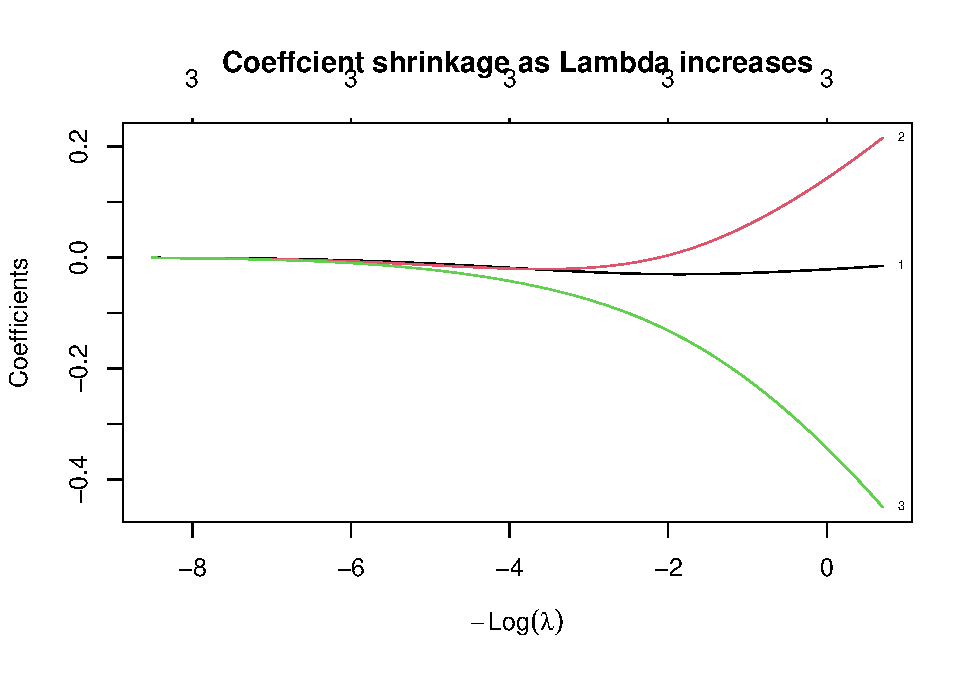
\includegraphics[width=1\linewidth]{skeleton-2_files/figure-latex/unnamed-chunk-7-1}

A smaller -log(\(\lambda\)) value indicates a larger penalty, therefore
our coefficients reduce to zero, as -log(\(\lambda\)) increases, our
coefficients move to their true values.

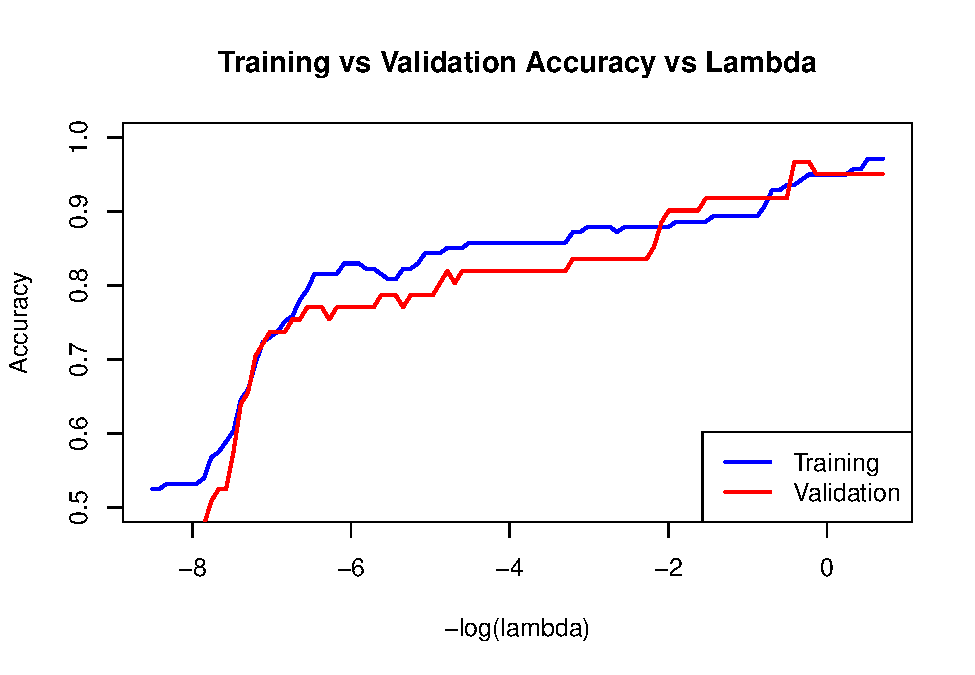
\includegraphics[width=1\linewidth]{skeleton-2_files/figure-latex/unnamed-chunk-8-1}

To evaluate the effect of the regularization parameter \(\lambda\) on
model performance, we computed predicted probabilities from both the
Ridge-IWLS model and glmnet logistic regression across a sequence of
\(\lambda\) values. For each \(\lambda\), the predicted probabilities
were converted into binary class predictions using a threshold of 0.5,
and accuracy was calculated separately on the training and validation
sets. This procedure allows us to observe how increasing \(\lambda\)
(stronger regularization) shrinks the coefficients, reducing variance
and preventing overfitting. Typically, training accuracy decreases as
\(\lambda\) increases due to the penalty constraining the model, while
validation accuracy initially rises to a peak at an optimal \(\lambda\)
before declining as over-regularization induces underfitting. This
analysis illustrates the bias--variance tradeoff and demonstrates how
ridge regularization improves generalization compared to unpenalized
logistic regression.

\subsection{Appendix}\label{appendix}

\begin{Shaded}
\begin{Highlighting}[]
\CommentTok{\# Global options for the document}
\NormalTok{knitr}\SpecialCharTok{::}\NormalTok{opts\_chunk}\SpecialCharTok{$}\FunctionTok{set}\NormalTok{(}
  \AttributeTok{echo =} \ConstantTok{FALSE}\NormalTok{,}
  \AttributeTok{warning =} \ConstantTok{FALSE}\NormalTok{,}
  \AttributeTok{message =} \ConstantTok{FALSE}\NormalTok{,}
  \AttributeTok{fig.pos =} \StringTok{\textquotesingle{}!ht\textquotesingle{}}\NormalTok{, }\CommentTok{\# ={-} Change this line}
  \AttributeTok{out.width =} \StringTok{\textquotesingle{}100\%\textquotesingle{}}\NormalTok{, }
  \AttributeTok{dpi =} \DecValTok{300}
\NormalTok{)}

\CommentTok{\# Load all required packages}
\FunctionTok{library}\NormalTok{(knitr)}
\FunctionTok{library}\NormalTok{(kableExtra)}
\FunctionTok{library}\NormalTok{(glmnet)}
\NormalTok{dat }\OtherTok{=} \FunctionTok{read.table}\NormalTok{(}\StringTok{\textquotesingle{}\textasciitilde{}/Desktop/template/Assignment\_Disease.txt\textquotesingle{}}\NormalTok{, }\AttributeTok{header =} \ConstantTok{TRUE}\NormalTok{)}
\FunctionTok{attach}\NormalTok{(dat)}
\NormalTok{Y }\OtherTok{=}\NormalTok{ dat}\SpecialCharTok{$}\NormalTok{DiseaseStatus}
\NormalTok{X }\OtherTok{=} \FunctionTok{as.matrix}\NormalTok{(}\FunctionTok{cbind}\NormalTok{(}\DecValTok{1}\NormalTok{, dat[, }\FunctionTok{c}\NormalTok{(}\StringTok{"Measurement1"}\NormalTok{, }\StringTok{"Measurement2"}\NormalTok{, }\StringTok{"Measurement3"}\NormalTok{)]))}
\NormalTok{n }\OtherTok{=} \FunctionTok{length}\NormalTok{(Y)}
\NormalTok{p }\OtherTok{=} \FunctionTok{ncol}\NormalTok{(X)}
\NormalTok{glm\_fit }\OtherTok{=} \ControlFlowTok{function}\NormalTok{(Y, X, }\AttributeTok{lambda =} \DecValTok{1}\NormalTok{, }\AttributeTok{eps =} \FloatTok{1e{-}6}\NormalTok{, }\AttributeTok{K =} \DecValTok{100}\NormalTok{) \{}
\NormalTok{  beta }\OtherTok{=} \FunctionTok{rep}\NormalTok{(}\DecValTok{0}\NormalTok{, p)}
  \ControlFlowTok{for}\NormalTok{ (iter }\ControlFlowTok{in} \DecValTok{1}\SpecialCharTok{:}\NormalTok{K) \{}
    
    \CommentTok{\# Linear predictor}
\NormalTok{    eta }\OtherTok{=} \FunctionTok{as.vector}\NormalTok{(X }\SpecialCharTok{\%*\%}\NormalTok{ beta)}
    
    \CommentTok{\# For logistic regression (binomial), use:}
\NormalTok{    mu }\OtherTok{=} \DecValTok{1} \SpecialCharTok{/}\NormalTok{ (}\DecValTok{1} \SpecialCharTok{+} \FunctionTok{exp}\NormalTok{(}\SpecialCharTok{{-}}\NormalTok{eta))}
    
    \CommentTok{\# Weights and z}
\NormalTok{    W }\OtherTok{=} \FunctionTok{diag}\NormalTok{(}\FunctionTok{as.vector}\NormalTok{(mu }\SpecialCharTok{*}\NormalTok{ (}\DecValTok{1} \SpecialCharTok{{-}}\NormalTok{ mu)), n, n)}
\NormalTok{    z }\OtherTok{=}\NormalTok{ eta }\SpecialCharTok{+}\NormalTok{ (Y }\SpecialCharTok{{-}}\NormalTok{ mu) }\SpecialCharTok{/}\NormalTok{ (mu }\SpecialCharTok{*}\NormalTok{ (}\DecValTok{1} \SpecialCharTok{{-}}\NormalTok{ mu))}
    
    \CommentTok{\# Lambda Scaling}
\NormalTok{    P }\OtherTok{=} \FunctionTok{diag}\NormalTok{(}\FunctionTok{rep}\NormalTok{(lambda }\SpecialCharTok{/}\NormalTok{ n, p))}
    
    \CommentTok{\# Ridge{-}IWLS updated}
\NormalTok{    XtWX }\OtherTok{=} \FunctionTok{t}\NormalTok{(X) }\SpecialCharTok{\%*\%}\NormalTok{ W }\SpecialCharTok{\%*\%}\NormalTok{ X}
\NormalTok{    XtWz }\OtherTok{=} \FunctionTok{t}\NormalTok{(X) }\SpecialCharTok{\%*\%}\NormalTok{ W }\SpecialCharTok{\%*\%}\NormalTok{ z}
\NormalTok{    beta\_new }\OtherTok{=} \FunctionTok{solve}\NormalTok{(XtWX }\SpecialCharTok{+} \DecValTok{2} \SpecialCharTok{*}\NormalTok{ lambda }\SpecialCharTok{*} \FunctionTok{diag}\NormalTok{(p), XtWz)}
    
    \CommentTok{\# Check convergence}
    \ControlFlowTok{if}\NormalTok{ (}\FunctionTok{sqrt}\NormalTok{(}\FunctionTok{sum}\NormalTok{((beta\_new }\SpecialCharTok{{-}}\NormalTok{ beta)}\SpecialCharTok{\^{}}\DecValTok{2}\NormalTok{)) }\SpecialCharTok{\textless{}}\NormalTok{ eps) }\ControlFlowTok{break}
\NormalTok{    beta }\OtherTok{=}\NormalTok{ beta\_new}
\NormalTok{  \}}
\NormalTok{  return }\OtherTok{=} \FunctionTok{list}\NormalTok{(}\AttributeTok{coefficients =}\NormalTok{ beta, }\AttributeTok{iterations =}\NormalTok{ iter, }\AttributeTok{converged =}\NormalTok{ (iter }\SpecialCharTok{\textless{}}\NormalTok{ K))}
\NormalTok{\}}
\NormalTok{fit }\OtherTok{=} \FunctionTok{glm\_fit}\NormalTok{(Y, X, }\AttributeTok{lambda =} \DecValTok{1}\NormalTok{)}
\NormalTok{fit\_glmnet }\OtherTok{=} \FunctionTok{glmnet}\NormalTok{(X[,}\SpecialCharTok{{-}}\DecValTok{1}\NormalTok{], Y, }\AttributeTok{family =} \StringTok{"binomial"}\NormalTok{, }\AttributeTok{alpha =} \DecValTok{0}\NormalTok{, }\AttributeTok{lambda =} \DecValTok{1}\SpecialCharTok{/}\NormalTok{n, }\AttributeTok{intercept =} \ConstantTok{TRUE}\NormalTok{, }\AttributeTok{standardize =} \ConstantTok{FALSE}\NormalTok{ )}
\CommentTok{\#Ridge IWLS coefficients}
\NormalTok{df }\OtherTok{\textless{}{-}} \FunctionTok{data.frame}\NormalTok{(}
  \AttributeTok{Estimate =}\NormalTok{ fit}\SpecialCharTok{$}\NormalTok{coefficients}
\NormalTok{)}
\FunctionTok{kable}\NormalTok{(df, }\AttributeTok{format =} \StringTok{"latex"}\NormalTok{, }\AttributeTok{booktabs =} \ConstantTok{FALSE}\NormalTok{, }\AttributeTok{caption =} \StringTok{"Ridge IWLS {-} Coefficient estimates."}\NormalTok{) }\SpecialCharTok{\%\textgreater{}\%}
  \FunctionTok{kable\_styling}\NormalTok{(}\AttributeTok{latex\_options =} \StringTok{"hold\_position"}\NormalTok{)}

\CommentTok{\# glmnet coefficients}
\NormalTok{coefs }\OtherTok{\textless{}{-}} \FunctionTok{as.matrix}\NormalTok{(}\FunctionTok{coef}\NormalTok{(fit\_glmnet))}
\NormalTok{df2 }\OtherTok{\textless{}{-}} \FunctionTok{data.frame}\NormalTok{(}
  \AttributeTok{Estimate =}\NormalTok{ coefs[, }\DecValTok{1}\NormalTok{]}
\NormalTok{)}
\FunctionTok{kable}\NormalTok{(df2, }\AttributeTok{format =} \StringTok{"latex"}\NormalTok{, }\AttributeTok{booktabs =} \ConstantTok{FALSE}\NormalTok{, }\AttributeTok{caption =} \StringTok{"Glmnet coefficient estimates."}\NormalTok{) }\SpecialCharTok{\%\textgreater{}\%}
  \FunctionTok{kable\_styling}\NormalTok{(}\AttributeTok{latex\_options =} \StringTok{"hold\_position"}\NormalTok{)}

\CommentTok{\# IWLS predictions}
\NormalTok{eta\_iwls }\OtherTok{=}\NormalTok{ X }\SpecialCharTok{\%*\%}\NormalTok{ fit}\SpecialCharTok{$}\NormalTok{coefficients}
\NormalTok{p\_iwls }\OtherTok{=} \DecValTok{1} \SpecialCharTok{/}\NormalTok{ (}\DecValTok{1} \SpecialCharTok{+} \FunctionTok{exp}\NormalTok{(}\SpecialCharTok{{-}}\NormalTok{eta\_iwls))}


\CommentTok{\# glmnet predictions}
\NormalTok{p\_glmnet }\OtherTok{=} \FunctionTok{predict}\NormalTok{(fit\_glmnet,X[,}\SpecialCharTok{{-}}\DecValTok{1}\NormalTok{], }\AttributeTok{type =} \StringTok{"response"}\NormalTok{, }\AttributeTok{s =} \DecValTok{1}\SpecialCharTok{/}\NormalTok{n)}

\CommentTok{\#mean squared error}
\NormalTok{mse\_iwls }\OtherTok{=} \FunctionTok{mean}\NormalTok{((Y }\SpecialCharTok{{-}}\NormalTok{ p\_iwls)}\SpecialCharTok{\^{}}\DecValTok{2}\NormalTok{)}
\NormalTok{mse\_glmnet }\OtherTok{=} \FunctionTok{mean}\NormalTok{((Y }\SpecialCharTok{{-}}\NormalTok{ p\_glmnet)}\SpecialCharTok{\^{}}\DecValTok{2}\NormalTok{)}


\NormalTok{pred\_df }\OtherTok{=} \FunctionTok{data.frame}\NormalTok{(}
  \AttributeTok{Obs =} \DecValTok{1}\SpecialCharTok{:}\DecValTok{10}\NormalTok{,}
  \AttributeTok{Actual =}\NormalTok{ Y[}\DecValTok{1}\SpecialCharTok{:}\DecValTok{10}\NormalTok{],}
  \AttributeTok{IWLS\_Pred =} \FunctionTok{round}\NormalTok{(p\_iwls[}\DecValTok{1}\SpecialCharTok{:}\DecValTok{10}\NormalTok{], }\DecValTok{4}\NormalTok{),}
  \AttributeTok{Glmnet\_Pred =} \FunctionTok{round}\NormalTok{(p\_glmnet[}\DecValTok{1}\SpecialCharTok{:}\DecValTok{10}\NormalTok{], }\DecValTok{4}\NormalTok{)}
\NormalTok{)}

\FunctionTok{kable}\NormalTok{(pred\_df, }\AttributeTok{format =} \StringTok{"latex"}\NormalTok{, }\AttributeTok{booktabs =} \ConstantTok{FALSE}\NormalTok{, }\AttributeTok{caption =} \StringTok{"Predicted probabilities: Ridge{-}IWLS vs. glmnet"}\NormalTok{) }\SpecialCharTok{\%\textgreater{}\%}
  \FunctionTok{kable\_styling}\NormalTok{(}\AttributeTok{latex\_options =} \StringTok{"hold\_position"}\NormalTok{, }\AttributeTok{position =} \StringTok{"center"}\NormalTok{)}
\NormalTok{perf }\OtherTok{\textless{}{-}} \FunctionTok{data.frame}\NormalTok{(}
  \AttributeTok{Model =} \FunctionTok{c}\NormalTok{(}\StringTok{"Ridge{-}IWLS"}\NormalTok{, }\StringTok{"glmnet"}\NormalTok{),}
  \AttributeTok{MSE =} \FunctionTok{c}\NormalTok{(}\FunctionTok{round}\NormalTok{(mse\_iwls, }\DecValTok{6}\NormalTok{), }\FunctionTok{round}\NormalTok{(mse\_glmnet, }\DecValTok{6}\NormalTok{)))}
  \FunctionTok{kable}\NormalTok{(perf, }\AttributeTok{format =} \StringTok{"latex"}\NormalTok{, }\AttributeTok{booktabs =} \ConstantTok{TRUE}\NormalTok{, }\AttributeTok{caption =} \StringTok{"Model performance comparison (MSE)"}\NormalTok{) }\SpecialCharTok{\%\textgreater{}\%}
  \FunctionTok{kable\_styling}\NormalTok{(}\AttributeTok{latex\_options =} \StringTok{"hold\_position"}\NormalTok{, }\AttributeTok{position =} \StringTok{"center"}\NormalTok{)}
\NormalTok{fit }\OtherTok{=} \FunctionTok{glmnet}\NormalTok{(X[,}\SpecialCharTok{{-}}\DecValTok{1}\NormalTok{], Y, }\AttributeTok{family =} \StringTok{"binomial"}\NormalTok{,}\AttributeTok{alpha =} \DecValTok{0}\NormalTok{, }\AttributeTok{intercept =} \ConstantTok{TRUE}\NormalTok{, }\AttributeTok{standardize =} \ConstantTok{FALSE}\NormalTok{)}
\FunctionTok{plot}\NormalTok{(fit, }\AttributeTok{xvar =} \StringTok{"lambda"}\NormalTok{, }\AttributeTok{label =} \ConstantTok{TRUE}\NormalTok{, }\AttributeTok{main =} \StringTok{\textquotesingle{}Coeffcient shrinkage as Lambda increases\textquotesingle{}}\NormalTok{)}

\FunctionTok{set.seed}\NormalTok{(}\DecValTok{2025}\NormalTok{)}

\CommentTok{\# Split into training and validation sets}
\NormalTok{index }\OtherTok{=} \FunctionTok{sample}\NormalTok{(}\DecValTok{1}\SpecialCharTok{:}\NormalTok{n, }\AttributeTok{size =} \FloatTok{0.7}\SpecialCharTok{*}\NormalTok{n)}
\NormalTok{X\_train }\OtherTok{=}\NormalTok{ X[index, ]}
\NormalTok{Y\_train }\OtherTok{=}\NormalTok{ Y[index]}
\NormalTok{X\_val }\OtherTok{=}\NormalTok{ X[}\SpecialCharTok{{-}}\NormalTok{index, ]}
\NormalTok{Y\_val }\OtherTok{=}\NormalTok{ Y[}\SpecialCharTok{{-}}\NormalTok{index]}

\CommentTok{\# Fit Ridge (alpha = 0) over a sequence of lambda values}
\NormalTok{fit }\OtherTok{=} \FunctionTok{glmnet}\NormalTok{(X\_train, Y\_train, }\AttributeTok{family =} \StringTok{"binomial"}\NormalTok{, }\AttributeTok{alpha =} \DecValTok{0}\NormalTok{, }\AttributeTok{standardize =} \ConstantTok{FALSE}\NormalTok{)}

\CommentTok{\# Lambda sequence}
\NormalTok{lambda\_seq }\OtherTok{=}\NormalTok{ fit}\SpecialCharTok{$}\NormalTok{lambda}
\NormalTok{n\_lambda }\OtherTok{=} \FunctionTok{length}\NormalTok{(lambda\_seq)}

\CommentTok{\# Initialize accuracy vectors}
\NormalTok{train\_acc }\OtherTok{=} \FunctionTok{numeric}\NormalTok{(n\_lambda)}
\NormalTok{val\_acc }\OtherTok{=} \FunctionTok{numeric}\NormalTok{(n\_lambda)}

\CommentTok{\# Compute training and validation accuracy for each lambda}
\ControlFlowTok{for}\NormalTok{ (i }\ControlFlowTok{in} \DecValTok{1}\SpecialCharTok{:}\NormalTok{n\_lambda) \{}
\NormalTok{  pred\_train }\OtherTok{=} \FunctionTok{predict}\NormalTok{(fit, }\AttributeTok{newx =}\NormalTok{ X\_train, }\AttributeTok{s =}\NormalTok{ lambda\_seq[i], }\AttributeTok{type =} \StringTok{"response"}\NormalTok{)}
\NormalTok{  pred\_val }\OtherTok{=} \FunctionTok{predict}\NormalTok{(fit, }\AttributeTok{newx =}\NormalTok{ X\_val, }\AttributeTok{s =}\NormalTok{ lambda\_seq[i], }\AttributeTok{type =} \StringTok{"response"}\NormalTok{)}
  
\NormalTok{  train\_acc[i] }\OtherTok{=} \FunctionTok{mean}\NormalTok{((pred\_train }\SpecialCharTok{\textgreater{}} \FloatTok{0.5}\NormalTok{) }\SpecialCharTok{==}\NormalTok{ Y\_train)}
\NormalTok{  val\_acc[i] }\OtherTok{=} \FunctionTok{mean}\NormalTok{((pred\_val }\SpecialCharTok{\textgreater{}} \FloatTok{0.5}\NormalTok{) }\SpecialCharTok{==}\NormalTok{ Y\_val)}
\NormalTok{\}}

\CommentTok{\# Plot}
\FunctionTok{plot}\NormalTok{(}\SpecialCharTok{{-}}\FunctionTok{log}\NormalTok{(lambda\_seq), train\_acc, }\AttributeTok{type =} \StringTok{"l"}\NormalTok{, }\AttributeTok{col =} \StringTok{"blue"}\NormalTok{, }\AttributeTok{lwd =} \DecValTok{2}\NormalTok{,}
     \AttributeTok{xlab =} \StringTok{"{-}log(lambda)"}\NormalTok{, }\AttributeTok{ylab =} \StringTok{"Accuracy"}\NormalTok{, }\AttributeTok{ylim =} \FunctionTok{c}\NormalTok{(}\FloatTok{0.5}\NormalTok{, }\DecValTok{1}\NormalTok{),}
     \AttributeTok{main =} \StringTok{"Training vs Validation Accuracy vs Lambda"}\NormalTok{)}
\FunctionTok{lines}\NormalTok{(}\SpecialCharTok{{-}}\FunctionTok{log}\NormalTok{(lambda\_seq), val\_acc, }\AttributeTok{col =} \StringTok{"red"}\NormalTok{, }\AttributeTok{lwd =} \DecValTok{2}\NormalTok{)}
\FunctionTok{legend}\NormalTok{(}\StringTok{"bottomright"}\NormalTok{, }\AttributeTok{legend =} \FunctionTok{c}\NormalTok{(}\StringTok{"Training"}\NormalTok{, }\StringTok{"Validation"}\NormalTok{),}
       \AttributeTok{col =} \FunctionTok{c}\NormalTok{(}\StringTok{"blue"}\NormalTok{, }\StringTok{"red"}\NormalTok{), }\AttributeTok{lwd =} \DecValTok{2}\NormalTok{)}
\end{Highlighting}
\end{Shaded}







\end{document}
